\documentclass{standalone}

\begin{document}
	
	L'objectif des Generative Adversarial Networks est d'entraîner à la fois un générateur et un classifieur. Le classifieur est entraîné à détecter les contrefaçons produites par le générateur, par rapport au jeu de données original. Le générateur est lui entraîné à essayer de berner le classifieur. En entraînant chacun à son tour, on obtient un générateur approximant la distribution réelle des données.
	
	\begin{figure}[H]
		\center
		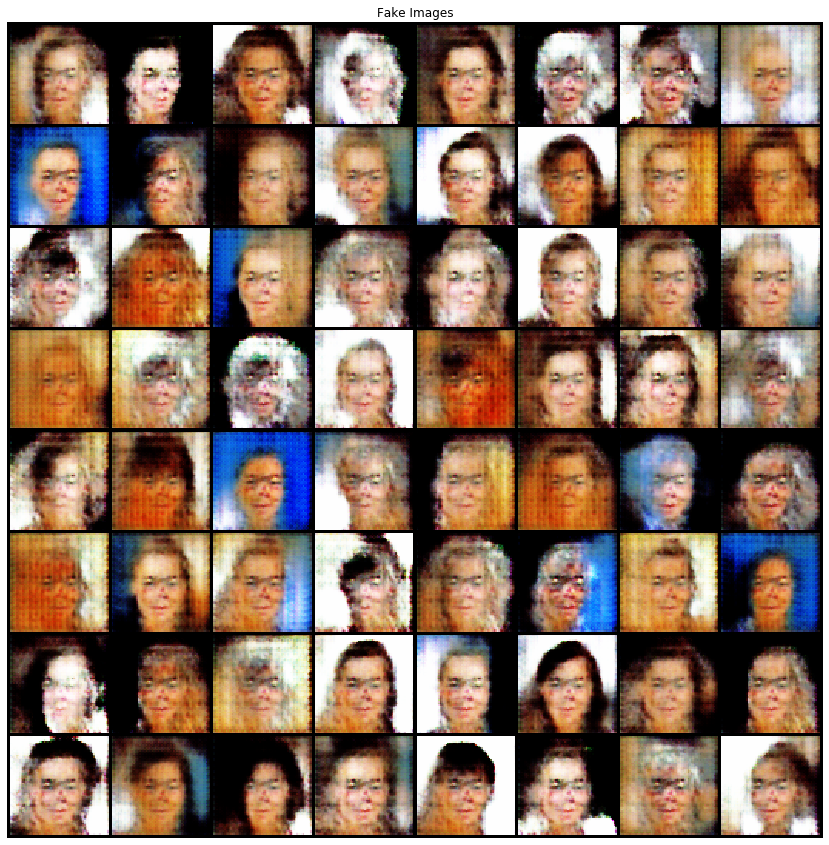
\includegraphics[scale=0.2]{img/faces2.png}
		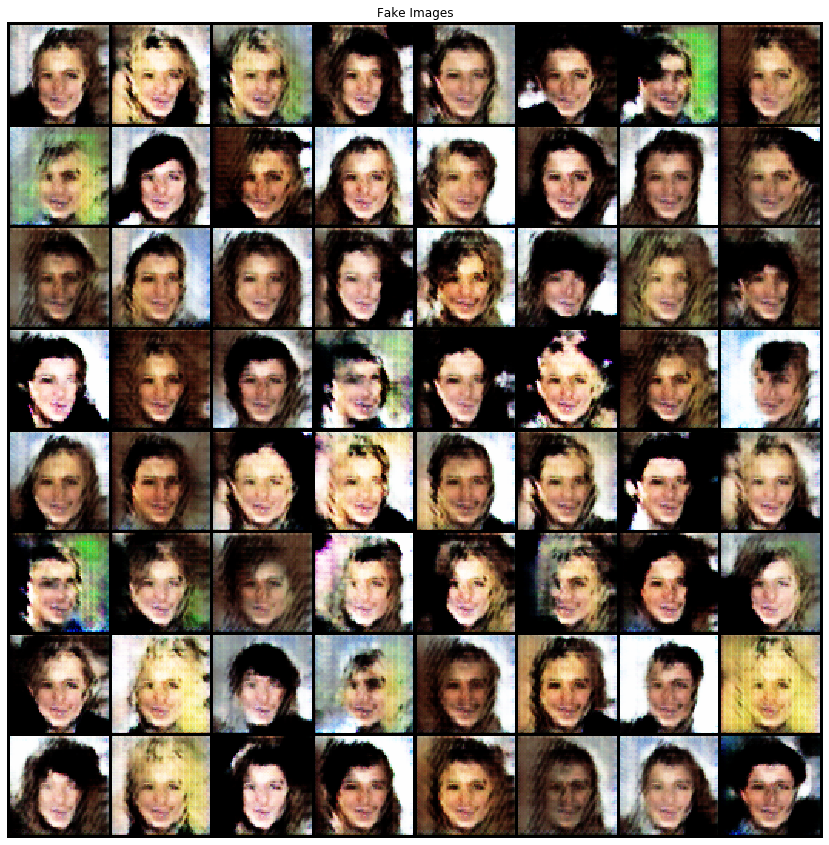
\includegraphics[scale=0.2]{img/faces3.png}
		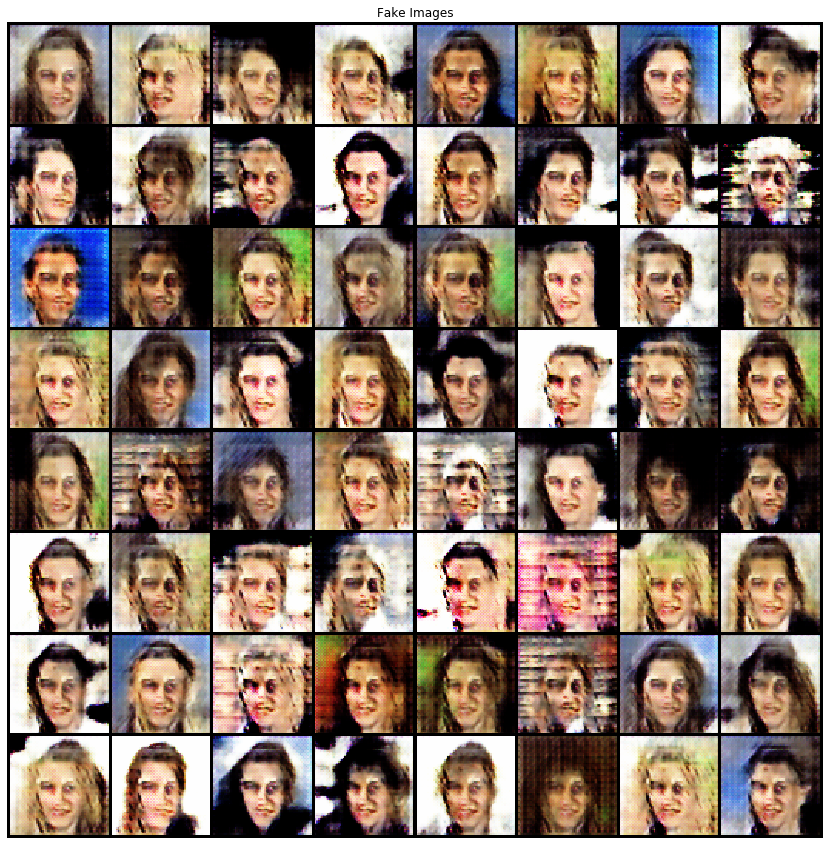
\includegraphics[scale=0.2]{img/faces4.png}
		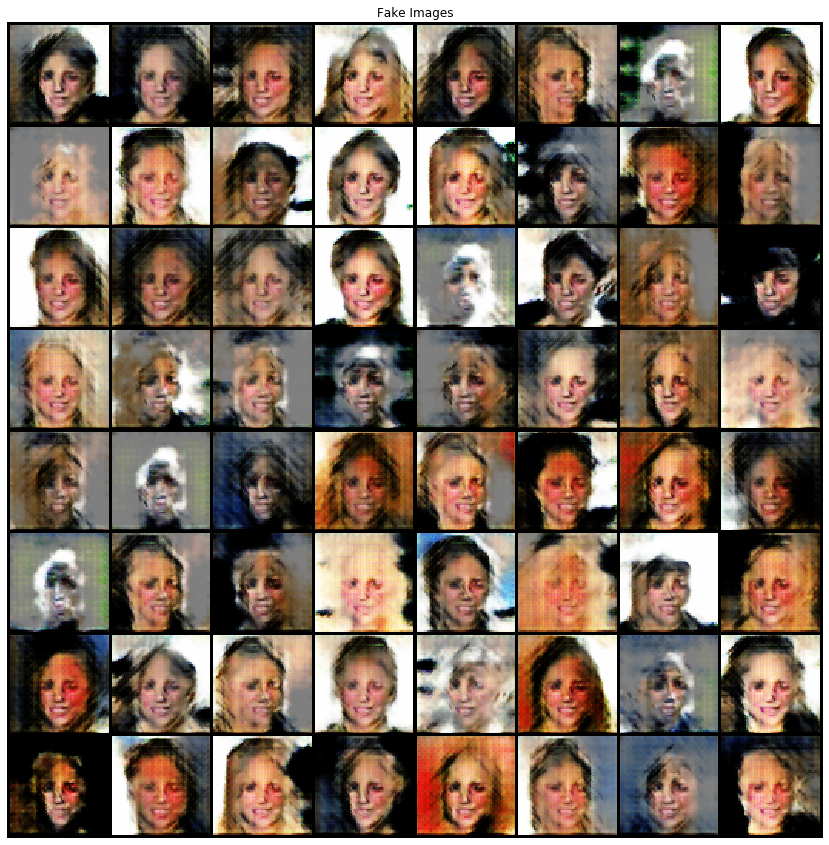
\includegraphics[scale=0.2]{img/faces5.png}
		\caption{Exemples de visages construits par le générateur au fur et à mesure de l'entraînement}
		\label{vae:samples}
	\end{figure}
\end{document}
